\documentclass[12pt,preprint]{aastex}
%\documentclass[12pt]{aastex}
\usepackage{graphicx}

\begin{document}



\title{OUR Z17 REDUCTION TECHNIQUE}

\author{Carl Heiles \today}
%\affil{Astronomy Department, University of California,
%    Berkeley, CA 94720-3411; cheiles@astron.berkeley.edu}

\begin{abstract}
We describe our observing technique and least-squares procedures to
determine the opacity profile, the expected emission profile, and their
uncertainty profiles. There are three procedures: \begin{enumerate}
\item {\tt z17\_1.pro}, which solves for the optical-depth profile, the
  expected profile, and the first-order Taylor expansion of the HI
  emission in the sky.
\item {\tt z17\_2.pro}, which solves for the optical-depth profile, the
  expected profile, and the second-order Taylor expansion of the HI
  emission in the sky.

\item {\tt fit\_z17.pro} fits for a second or third order Taylor expansion
  and does not use the cold-sky antenna temp (called trcvr) in the
  fit. Rather, it assumes the continuum source contributes zero to the
  system temperature when you are not at the on position. This is
  probably better because trcvr is not predicted perfectly
  accurately. However, deteremining which is better needs some
  experimentation. The baselines probably need to be subtracted before
  using {\tt fit\_z17}---needs checking!

\end{enumerate}
\S \ref{versus} discusses the differences between the latter two and which
might be preferable for particular cases.
\end{abstract}

\subsection{The Arecibo telescope and our Z17 Observing Pattern}

	The Arecibo telescope has a reflector fixed on the ground and
points by moving the feed structure.  This makes many characteristics of
the beam change as a source is tracked.  These changes are discussed by
Heiles et al.\ (2001) and documented in more detail on Arecibo's website.
We sampled two linearly polarized channels simultaneously, performing
both auto and crosscorrelations with Arecibo's three-level ``interim''
digital correlator. 

We observed each source by repeating our observational pattern.  This
pattern consists of 17 positions: one on-source and
16 off-source positions (Figure \ref{crossfig}).  It allows us to
calculate and correct for the first and second derivatives of 21-cm line
emission intensity on the sky. With 17 positions, we refer to
this pattern as ``Z17''.

\begin{figure}[h!]
\begin{center}
\includegraphics[width=3.5in] {f1.ps} 
%\leavevmode
%\epsfxsize=5in
%\epsffile{cross.ps}
\end{center}
\caption{The 17-point measurement grid of the Z16 pattern. It consists
of two crosses, one aligned with ra/dec (squares) and one at $45^\circ$
to ra/dec (diamonds).  The innermost points are $1.0 \, H\!P\!B\! W$ and
the outermost points $2^{1/2} H\!P\!B\!W$ from the central point. 
\label{crossfig}} \end{figure}

In addition to the spatial derivatives, there are instrumental effects
involving the system gain. The on-source antenna temperature can vastly
exceed the off-source ones.  With three-level correlators it is
important to keep the input level near the optimum value; this meant
that the electronics gains for the on-source measurements (${\cal G}_n$
below) were set lower than those for the off-source ones ($G_n$ below).
These gains had to be calibrated independently and have independent
uncertainties. The instrumental effects
that should be accounted for include: \begin{enumerate}

\item The on-source electronics gain ${\cal G}$ for each pattern
$n$ is not perfectly calibrated. 

\item The off-source electronics gain $G$ for each pattern $n$ is not
perfectly calibrated. 

\item The on-axis gain of the telescope changes with $(az,za)$, so that
the source deflection changes. 

\item Arecibo's beam shape changes with $(az,za)$.  In particular, the
location of the first zero in the antenna beam response changes and,
moreover, does not always exist.  This means that the off-source spectra
contain some remnant of the source intensity so one cannot obtain the
expected profile by going just a little way off source. 

\item The intrinsic system temperature changes with $za$, particularly
  at high $za$ where the feed response spills over to onto the ground. 

\end{enumerate}

In the reductions for the Millennium survey (Heiles \& Troland 2003), we
accounted for all of these effects. Here, we use a simpler reduction
technique, which only accounts for the last two above.  We ignore the
first three because the on-axis gain changes with $(az,za)$; accounting
for it requires
knowledge of the telescope gain and beam properties, which in any case
are somewhat uncertain and also can change as the telescope surface
errors increase gradually with time, or decrease when adjusted. We feel
that the associated uncertainties make HT's original technique
``overkill''.

However, the fourth instrumental effect, the telescope's off-axis
point-source response, is easy to evaluate from the off-line spectral
baseline channels. And the fifth, the change in system temperature with
$za$, depends only on the spillover onto the ground; this depends only
on illumination pattern on the primary surface, which, in turn, depends
only on the feed illumination pattern and the arrangement of the
subreflectors. This means that this effect is stable in time. Moreover,
it is easy to correct for.

\subsection{ Our Simpler Analysis Technique}

To derive 21-cm absorption line spectra, one observes off-source
positions to obtain the ``expected profile'' $T_{E}(\nu )$, which is the
line profile one would observe at the source's position if the continuum
source were turned off. One uses the expected profile for two purposes:
one subtracts it from the on-source spectrum, which difference provides
the opacity spectrum; and one combines it with the opacity spectrum to
obtain the spin temperatures.

	This conventional technique is not perfect because the
off-source emission spectra differ from the expected profile. There are
two reasons. First, the antenna response to the continuum source is not
zero for the off positions, so the off-source emission spectra are
contaminated by a small, unknown contribution from the opacity spectrum.
Second, there is angular structure in the emission spectra. We treat these
problems using a least squares technique.

We assume that the angular structure in each spectral channel can be
represented by a Taylor series expansion. The Z17 pattern allows us to
evaluate this expansion to second order. Within each pattern we have $J$
measurements, each of which is denoted by subscript $j$. Each pattern
consists of measurements at $J=17$ positions, one of which is directly
on-source; even the off-source positions have nonzero
antenna temperature from the source, as discussed above.
The symbols $(\nu)$ indicate frequency-dependent quantities within the
profile; unsubscripted temperatures are continuum.  Quantities to be
derived from a least squares treatment are enclosed in square brackets.
There are 7 such quantities for the full second-order expansion and 4
for the first-order one.

Thus, for each pattern we have the equations of condition

\begin{equation} \label{ls1}
T_{A,j}(\nu) - T_{R,j} = [e^{-\tau (\nu)}] T_{C,j}  + [T_{E}(\nu)] +
\left[ \partial T_{E}(\nu) \over \partial \alpha \right] \Delta\alpha_{j} + 
\left[ \partial T_{E}(\nu) \over \partial \delta \right] \Delta\delta_{j} + $$
$$
\left[ \partial^2 T_{E}(\nu) \over \partial \alpha^2 \right]
     {(\Delta\alpha_{j})^2 \over 2} + 
\left[ \partial^2 T_{E}(\nu) \over \partial \delta^2 \right]
     {(\Delta\delta_{j})^2 \over 2} + 
\left[ \partial^2 T_{E}(\nu) \over \partial\alpha \partial\delta \right]
     (\Delta\alpha_{j}) \ (\Delta\delta_{j}) \ ,
\end{equation}

\noindent where $T_{A,j}(\nu)$ are the measured antenna temperatures,
$T_{R,j}$ are the receiver temperatures (a function of $za$),
$T_{E}(\nu)$ is the 21-cm line emission that would be observed in the
absence of the source,  $\Delta \alpha_j$ are
the right-ascension offsets, and $\Delta \delta_j$ are
the declination offsets. 

$T_{C,j}$ are the antenna temperatures of the source
(which are small except at the on-source position). We obtain these from
the off-line ``baseline'' spectral channels.

\subsection{First-order versus Second-order Taylor Expansion \label{versus}} 

There are two reduction programs. {\tt z17\_1.pro} solves for the
first-order expansion, and {\tt z17\_2.pro} solves for the second order
one. We recommend using both, comparing the results, and using the
appropriate one for each particular case. 

In principle, the second-order Taylor expansion is preferred because it
can more accurately represent the true spatial variation of
$T_E(\nu)$. However, its derived spectra for both $T_E(\nu)$ and 
$e^{-\tau (\nu)}$ are noisier than those derived from the first-order
Taylor expansion. The excess noise occurs for two
reasons:. \begin{enumerate}

\item In the second-order expansion there are $P=6$ unknown parameters
  derived from $M=17$ measurements, in contrast to the first-order one
  where there are only $P=3$ unknowns. The statistical noise is
  proportional to $(M-P)^{-1/2}$, so the former expansion is
  intrinsically noisier by $(14/11)^{1/2} = 1.13$. 

\item More serious is the high covariance between the second derivatives
  of the expected profile and the $e^{-\tau (\nu)}$ and $T_{E}(\nu)$
  spectra. For the second-order expansion, the typical normalized
  covariance matrix (also known as the correlation matrix) for the
  unknowns in equation \ref{ls1} is

\begin{eqnarray} \label{ncov2}
{\bf ncov2} = \left[
\begin{array}{rrrrrrr}
  1.00 & -0.34  & 0.02 & -0.00 &  0.55 &  0.55 &  0.00 \\
 -0.34 &  1.00 & -0.01 &  0.00 & -0.82 & -0.82 & -0.00 \\
  0.02 & -0.01  & 1.00 & -0.00 &  0.01 &  0.01 &  0.00 \\
 -0.00 &  0.00  & -0.00 &  1.00 & -0.00 & -0.00 &  0.00 \\
  0.55 & -0.82  & 0.01 & -0.00 &  1.00 &  0.67 &  0.00 \\
  0.55 & -0.82  & 0.01 & -0.00 &  0.67 &  1.00 &  0.00 \\
  0.00 & -0.00  & 0.00 &  0.00 &  0.00 &  0.00 &  1.00 
\end{array}
\right]
\end{eqnarray} 

\noindent while that for the first-order expansion is

\begin{eqnarray} \label{ncov1}
{\bf ncov1} = \left[
\begin{array}{rrrr}
  1.00 &  0.56 &  0.01 & -0.00 \\
  0.56 &  1.00 &  0.01 & -0.00 \\
  0.01 &  0.01 &  1.00 & -0.00 \\
 -0.00 & -0.00 & -0.00 &  1.00 
\end{array}
\right]
\end{eqnarray} 

\noindent The matrix {\bf ncov2} exhibits high covariance (--0.82)
between the interesting parameters ($T_E(\nu)$ and $e^{-\tau (\nu)}$)
and the second derivatives ($\partial^2 T_{E}(\nu) \over \partial
\alpha^2$ and $\partial^2 T_{E}(\nu) \over \partial \delta^2$). This
contributes to the statistical noise.

\end{enumerate}

Thus, we have a tradeoff: the second-order expansion is more accurate
(smaller systematic errors), while the first-order one is more precise
(smaller random errors).  We illustrate these points with our results for
a single pattern for 3C132. Figure \ref{3c132fig}. For $e^{-\tau
  (\nu)}$, the black (first order) and red (second order) fits differ
significantly near $Vlsr=15$ km/s; the second order fit should be more
accurate.

\begin{figure}[h!]
\begin{center}
\includegraphics[scale=0.75] {z17mstst.ps} 
\end{center}
\caption{First-order (black) and second-order (red) fits for the
  $T_E(\nu)$ (bottom) and $e^{-\tau (\nu)}$ (top) profiles for
  3C132. \label{3c132fig}} \end{figure}



\begin{references}

\reference {} Heiles, C.\ et al.\ 2001, \pasp, 113, 1247.

\reference {} Heiles, C.\ \& Troland, T.H.\ 2003, ApJS, 145, 329

\end{references}

\end{document}

